%% For normal draft builds (figs undisplayed hence fast compile)
%\documentclass[hyperpdf,nobind,draft,oneside]{hepthesis}
%\documentclass[hyperpdf,nobind,draft,twoside]{hepthesis}

%% For short draft builds (breaks citations by necessity)
%\documentclass[hyperpdf,nobind,draft,hidefrontback]{hepthesis}

%%For Cambridge soft-bound version
\documentclass[hyperpdf,bindnopdf]{hepthesis}
%% For Cambridge hard-bound version (must be one-sided)
%\documentclass[hyperpdf,oneside]{hepthesis}

%% Load special font packages here if you wish
%\usepackage{lmodern}
\usepackage{mathpazo}
%\usepackage{euler}

%% Put package includes etc. into preamble.tex for convenience
\usepackage{xspace}
\usepackage{tikz}
\usepackage{morefloats,subfig,afterpage}
\usepackage{mathrsfs} % script font
\usepackage{verbatim}

%% Using Babel allows other languages to be used and mixed-in easily
%\usepackage[ngerman,english]{babel}
\usepackage[english]{babel}
\selectlanguage{english}

%% Citation system tweaks
\usepackage{cite}
% \let\@OldCite\cite
% \renewcommand{\cite}[1]{\mbox{\!\!\!\@OldCite{#1}}}

%% Maths
% TODO: rework or eliminate maybemath
\usepackage{abmath}
\DeclareRobustCommand{\mymath}[1]{\ensuremath{\maybebmsf{#1}}}
% \DeclareRobustCommand{\parenths}[1]{\mymath{\left({#1}\right)}\xspace}
% \DeclareRobustCommand{\braces}[1]{\mymath{\left\{{#1}\right\}}\xspace}
% \DeclareRobustCommand{\angles}[1]{\mymath{\left\langle{#1}\right\rangle}\xspace}
% \DeclareRobustCommand{\sqbracs}[1]{\mymath{\left[{#1}\right]}\xspace}
% \DeclareRobustCommand{\mods}[1]{\mymath{\left\lvert{#1}\right\rvert}\xspace}
% \DeclareRobustCommand{\modsq}[1]{\mymath{\mods{#1}^2}\xspace}
% \DeclareRobustCommand{\dblmods}[1]{\mymath{\left\lVert{#1}\right\rVert}\xspace}
% \DeclareRobustCommand{\expOf}[1]{\mymath{\exp{\!\parenths{#1}}}\xspace}
% \DeclareRobustCommand{\eexp}[1]{\mymath{e^{#1}}\xspace}
% \DeclareRobustCommand{\plusquad}{\mymath{\oplus}\xspace}
% \DeclareRobustCommand{\logOf}[1]{\mymath{\log\!\parenths{#1}}\xspace}
% \DeclareRobustCommand{\lnOf}[1]{\mymath{\ln\!\parenths{#1}}\xspace}
% \DeclareRobustCommand{\ofOrder}[1]{\mymath{\mathcal{O}\parenths{#1}}\xspace}
% \DeclareRobustCommand{\SOgroup}[1]{\mymath{\mathup{SO}\parenths{#1}}\xspace}
% \DeclareRobustCommand{\SUgroup}[1]{\mymath{\mathup{SU}\parenths{#1}}\xspace}
% \DeclareRobustCommand{\Ugroup}[1]{\mymath{\mathup{U}\parenths{#1}}\xspace}
% \DeclareRobustCommand{\I}[1]{\mymath{\mathrm{i}}\xspace}
% \DeclareRobustCommand{\colvector}[1]{\mymath{\begin{pmatrix}#1\end{pmatrix}}\xspace}
\DeclareRobustCommand{\Rate}{\mymath{\Gamma}\xspace}
\DeclareRobustCommand{\RateOf}[1]{\mymath{\Gamma}\parenths{#1}\xspace}

%% High-energy physics stuff
\usepackage{abhep}
\usepackage{hepnames}
\usepackage{hepunits}
\DeclareRobustCommand{\arXivCode}[1]{arXiv:#1}
\DeclareRobustCommand{\CP}{\ensuremath{\mathcal{CP}}\xspace}
\DeclareRobustCommand{\CPviolation}{\CP-violation\xspace}
\DeclareRobustCommand{\CPv}{\CPviolation}
\DeclareRobustCommand{\LHCb}{LHCb\xspace}
\DeclareRobustCommand{\LHC}{LHC\xspace}
\DeclareRobustCommand{\LEP}{LEP\xspace}
\DeclareRobustCommand{\CERN}{CERN\xspace}
\DeclareRobustCommand{\bphysics}{\Pbottom-physics\xspace}
\DeclareRobustCommand{\bhadron}{\Pbottom-hadron\xspace}
\DeclareRobustCommand{\Bmeson}{\PB-meson\xspace}
\DeclareRobustCommand{\bbaryon}{\Pbottom-baryon\xspace}
\DeclareRobustCommand{\Bdecay}{\PB-decay\xspace}
\DeclareRobustCommand{\bdecay}{\Pbottom-decay\xspace}
\DeclareRobustCommand{\BToKPi}{\HepProcess{ \PB \to \PK \Ppi }\xspace}
\DeclareRobustCommand{\BToPiPi}{\HepProcess{ \PB \to \Ppi \Ppi }\xspace}
\DeclareRobustCommand{\BToKK}{\HepProcess{ \PB \to \PK \PK }\xspace}
\DeclareRobustCommand{\BToRhoPi}{\HepProcess{ \PB \to \Prho \Ppi }\xspace}
\DeclareRobustCommand{\BToRhoRho}{\HepProcess{ \PB \to \Prho \Prho }\xspace}
\DeclareRobustCommand{\X}{\thesismath{X}\xspace}
\DeclareRobustCommand{\Xbar}{\thesismath{\overline{X}}\xspace}
\DeclareRobustCommand{\Xzero}{\HepGenParticle{X}{}{0}\xspace}
\DeclareRobustCommand{\Xzerobar}{\HepGenAntiParticle{X}{}{0}\xspace}
\DeclareRobustCommand{\epluseminus}{\Ppositron\!\Pelectron\xspace}
\DeclareRobustCommand{\protonproton}{\Pproton\APantiproton\xspace}


%% You can set the line spacing this way
%\setallspacing{double}
%% or a section at a time like this
%\setfrontmatterspacing{double}


%% Define the thesis title and author
\title{A study of \BToKPi decays with\\ the \LHCb experiment}
\author{Andrew Gordon Buckley}

%% Doc-specific PDF metadata
\makeatletter
\@ifpackageloaded{hyperref}{%
\hypersetup{%
  pdftitle = {Studying B to K pi decays with LHCb},
  pdfsubject = {Andy Buckley's PhD thesis},
  pdfkeywords = {LHCb, B, physics, LHC, heavy flavour},
  pdfauthor = {\textcopyright\ Andy Buckley}
}}{}
\makeatother


%% Start the document
\begin{document}

%% Define the un-numbered front matter (cover pages, rubrik and table of contents)
\begin{frontmatter}
  %% Title
%!!UPDATE THIS
\titlepage[of Imperial College London]%
{A dissertation submitted to Imperial College London\\
  for the degree of Doctor of Philosophy}
  
\clearpage
\textbf{The copyright of this thesis rests with the author and is made available under a Creative Commons 
Attribution Non-Commercial No Derivatives licence. Researchers are free to copy, distribute or 
transmit the thesis on the condition that they attribute it, that they do not use it for commercial 
purposes and that they do not alter, transform or build upon it. For any reuse or redistribution, 
researchers must make clear to others the licence terms of this work.}


%% Abstract
\begin{abstract}%[\smaller \thetitle\\ \vspace*{1cm} \smaller {\theauthor}]
The Compact Muon Solenoid (CMS) is a general-purpose particle detector at the CERN Large Hadron Collider (LHC). The goal of this experiment is to search for the Higgs boson and evidence of new physics and to test the prediction of the Standard Model (SM) at the TeV scale. This thesis describes the analysis of proton-proton collision data recorded by CMS during 2012 and support work for data taking during the same period.

A search for the Vector Boson Fusion (VBF) produced Higgs boson invisible decays, using $19.5\,\femto\barn^-1$ of data recorded with prompt reconstruction triggers at a center of mass energy of $8\,\TeV$, is presented. Events are selected with two forward jets and large Missing Transverse Momentum. Assuming the SM VBF production cross section and acceptance, the observed (expected) upper limit at the 95\% confidence level on the \BRinv\, is determined to be of 65\% (49\%) for $m_H=125\,\GeV$.

A second search for the VBF Higgs boson invisible decays, using $19.2\,\femto\barn^-1$ of data recorded with delayed reconstruction (parked) triggers at a center of mass energy of $8\,\TeV$, is also presented. A new event selection criteria was developed taking advantage of the lower trigger requirements. Assuming the SM VBF Higgs production cross section and acceptance, the observed (expected) upper limit at the 95\% confidence level on the \BRinv\, is determined to be of 57\% (40\%) for $m_H=125\,\GeV$.

Monitoring for the CMS Level 1 Trigger system has been developed and used during the 2012 and subsequent LHC data acquisition periods. Contribution to the high reliability of this system during data taking and providing crucial information for validation of the data quality.
\end{abstract}

%DONE

%% Declaration
\begin{declaration}
I declare that the work contained in this thesis is my own, and all results and figures taken from other sources are indicated in the text and referenced appropriately. The analyses presented in this thesis were developed in close collaboration with other members of the CMS experiment.

For the Vector Boson Fusion (VBF) Higgs to invisible prompt analysis I have contributed with the literature review and final background cross section input values for background normalization. QCD multi-jet background studies were also preformed with the target of improving the final selection or prepare the parked analysis, this analysis is presented to give context for the more important work developed later. 

For the VBF Higgs to invisible parked analysis I have participated in the development of the parked trigger, which was used to record the majority of the analysed data. I have continued the QCD multi-jet background studies which have lead to the production of dedicated Monte Carlo simulations and novel approaches to reject this type of events. I have been the responsible for the cross check analysis of the main result which has successfully validated the implementation of the main analysis \cite{ARTICLE:CMSVBFHiggsInvisibleParkedAnalysisPAS}. It is a normal a requirement for many \gls{CMS} publications to have a cross check analysis implemented independently from the main result in order to be able to ensure the accuracy of the final results. I have also participated in the preparation of the Run II analysis where I have lead the development of both the triggers used for data recording during 2015. Additionally, I have developed a method to create the first QCD multi-jet Monte Carlo sample with no MET requirements with signal like properties.

As part of the CMS Level 1 Trigger (L1T) Detector Performance Group (DPG) I have developed monitoring tools for this system, which were both used for real-time monitoring and posterior data certification for physics analysis usage. My work in this group has lead to my appointment for two years to the position of coordinator of the \gls{CMS} \gls{L1T} Data quality Monitoring software development team. Field work was also performed by doing shifts as Trigger and Shift Leader in the experiment control room and on call shifts as the Trigger Detector on Call (DOC) expert.
 
\vspace*{1cm}
\begin{flushright}
João Pela
\end{flushright}
\end{declaration}

%% Acknowledgements
\begin{acknowledgements}
I would like to thank the Imperial College HEP Group and the FCT for supporting and giving me the opportunity to pursue research including my time spent at CERN. Thanks to my supervisor, David Colling, for his guidance during the years of my PhD, the many useful discussions and his enthusiasm for particle physics research. Thanks must also go to all my colleagues of the CMS VBF Higgs to invisible group with whom I have worked directly, Patrick Dunne, Anne-Marie Magnan, Alexandre Nikitenko, Jim Brooke and Chayanit Asawatangtrakuldee. Thanks to everyone in CMS L1T DPG group, specially to Carlo Battilana and Arno Heister for their support. Thanks to all my friends that supported me on my way to finish this degree, it is difficult to mention all of you, but here is a small list, Antonio Pacheco, André David, Alice Mitchell, Chris Holdsworth-Swan, Francisco Sousa, Glenn Spiers, Guillermo Marrero, João Filipe, Miguel Cunhal, Miguel Machado, Nadia Silva, Raquel Monteiro, and many, many more. Finally, and most importantly, I thank my parents and grandparents for their constant support, love and encouragement.
\end{acknowledgements}

\clearpage

\vspace*{\fill}
The work presented in this thesis was supported by the Portuguese Government through \gls{FCT} in the form of my PhD grant with the reference SFRH/BD/77979/2011. I am thankful for their support which allowed me to attain higher education.
\vspace*{\fill}

\begin{center}
\resizebox{1.0\linewidth}{!}{

\includegraphics{FrontMatter/Images/FundingBand.png}
}
\end{center}


% \begin{preface}
% Thesis structure and so on...
% \end{preface}

\dedication{To my grandmother.}

%% Preface
%\begin{preface}
%\end{preface}

%% ToC
\tableofcontents

\newpage
\listoffigures

\newpage
\listoftables

%% Strictly optional!
%\frontquote%
%{Writing in English is the most ingenious torture\\
%   ever devised for sins committed in previous lives.}%
%  {James Joyce}
 
% \titlepage[of the High Energy Physics Group]{%
%   A dissertation submitted to the Imperial College London\\ for the degree of Doctor of Philosophy}

\end{frontmatter}

%% Start the content body of the thesis
\begin{mainmatter}
  %% Actually, more semantic chapter filenames are better, like "chap-bgtheory.tex"
  \chapter{\CP violation in the \Bmeson system}
\label{chap:SomeStuff}

%% Restart the numbering to make sure that this is definitely page #1!
\pagenumbering{arabic}

%% Note that the citations in this chapter use the journal and
%% arXiv keys: I used the SLAC-SPIRES online BibTeX retriever
%% to build my bibliography. There are also quite a few non-standard
%% macros, which come from my personal collection. You can have them
%% if you want, or I might get round to properly releasing them at
%% some point myself.

\chapterquote{Laws were made to be broken.}%
{Christopher North, 1785--1854}%: Blackwood's Magazine May 1830

Symmetries, either intact or broken, have proved to be at the heart
of how matter interacts. The Standard Model of fundamental interactions
(SM) is composed of three independent continuous symmetry groups denoted
$\SUgroup{3} \times \SUgroup{2} \times \Ugroup{1}$, representing the
strong force, weak isospin and hypercharge
respectively~\cite{Phys.Rev.Lett.19.1264, Phys.Rev.D2.1285,hep-ph/0410370}.

\section{Neutral meson mixing}
\label{sec:neutralmixing}
We can go a long way with an effective Hamiltonian approach in
canonical single-particle quantum mechanics. To do this we construct
a wavefunction from a combination of a generic neutral meson state
$\ket{\Xzero}$ and its anti-state $\ket{\Xzerobar}$:
%
\begin{equation}
  \ket{\psi(t)} = a(t)\ket{\Xzero} + b(t)\ket{\Xzerobar}
\end{equation}
%
which is governed by a time-dependent matrix differential equation,
%
\begin{equation}
  \I \pdByd{}{t} \colvector{a \\ b}
  =
  \underbrace{%
  \twomatrix{ M_{11}-\frac{\I}{2}\Gamma_{11}
            & M_{12}-\frac{\I}{2}\Gamma_{12} }
            { M_{12}^\ast-\frac{\I}{2}\Gamma_{12}^\ast
            & M_{22}-\frac{\I}{2}\Gamma_{22} }
  }_{\boldmatrix{H}}
  \colvector{a \\ b}
  .
\end{equation}

  \chapter{The \LHCb experiment}
\label{chap:MoreStuff}

\chapterquote{There, sir! that is the perfection of vessels!}
{Jules Verne, 1828--1905}

\section{The \LHC}
The Large Hadron Collider (\LHC) at \CERN is a new hadron collider,
located in the same tunnel as the Large Electron-Positron collider
(\LEP)~\cite{Brianti:2004qq}. Where \LEP's chief task was the use
of \unit{90--207}{\GeV} \epluseminus collisions to establish the
precision physics of electroweak unification\dots

% \begin{figure}
%   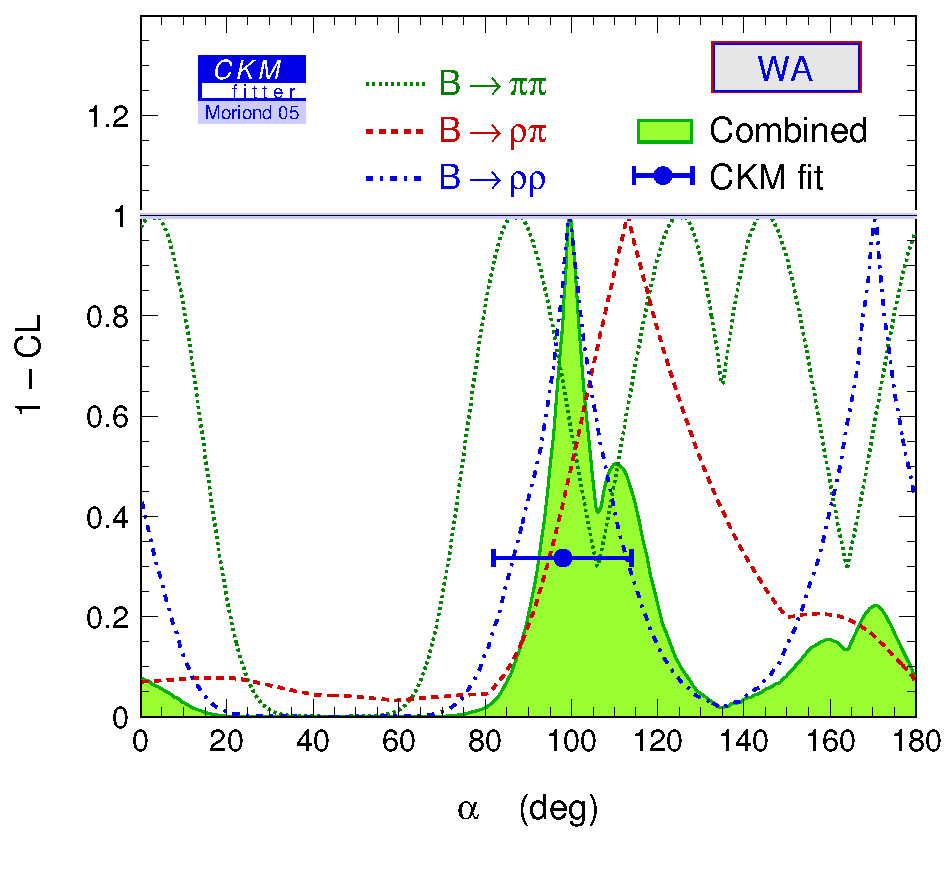
\includegraphics[width=\largefigwidth]{ckmfitter-alpha-combined}
%   \caption[CKM Fitter constraints on \alphaCKM.]%
%   {CKM Fitter constraints on \alphaCKM from combined \BToPiPi,
%     \BToRhoPi and \BToRhoRho decay analyses.}
%   \label{fig:CKMFitter}
% \end{figure}

\section{The \LHCb experiment}
\label{sec:LHCbInDetail}

Since both \bhadron{s} are preferentially produced in the same direction
and are forward-boosted along the beam-pipe, the detector is not required
to have full $4\pi$ solid-angle coverage. \LHCb takes advantage of this
by using a wedge-shaped single-arm detector with angular acceptance
\unit{10-300}{\mrad} in the horizontal (bending) plane~\cite{Amato:1998xt}.

\vspace{1cm}

\begin{center}
{\hspace{1mm}\Large\vdots\hspace{1cm}}
\end{center}

\vspace{1cm}

The detector is illustrated in \FigureRef{fig:LHCbCrossSection}, showing
the overall scale of the experiment and the surrounding cavern structure.

\begin{sidewaysfigure}
  \begin{center}
  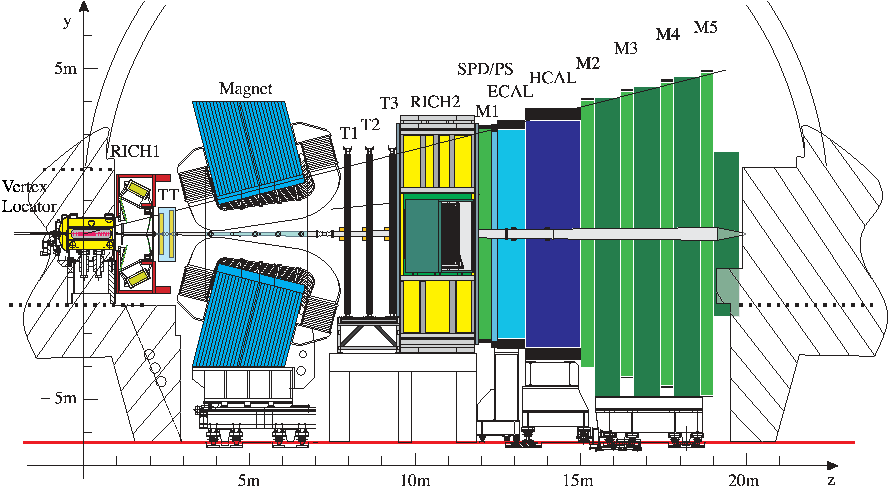
\includegraphics[width=0.8\textheight]{lhcb-detector-cross-section}
  \caption[Cross-section view of \LHCb, cut in the non-bending $y$--$z$ plane]%
    {Cross-section view of \LHCb, cut in the non-bending $y$--$z$ plane.}
  \label{fig:LHCbCrossSection}
  \end{center}
\end{sidewaysfigure}

The single-sided detector design was chosen in preference to a two-armed
design since the detector dimensions are restricted by the layout of the
IP8 (ex-Delphi) cavern in which \LHCb is located. Using all the available
space for a single-arm spectrometer more than compensates in performance
for the \about{50\percent} drop in luminosity.

\section{The \Cerenkov mechanism}
A Huygens construction in terms of spherical shells of probability for photon
emission as the particle progresses along its track shows an effective
``shock-front'' of \Cerenkov emission. This corresponds to an emission cone of
opening angle \thetaCerenkov around the momentum vector for each point on the
track,
%
\begin{subequations}
  \label{eq:cosThetaCk}
  \begin{equation}
    \cos\,\thetaCerenkov  &= \frac{1}{n \beta} +
                             \frac{\hbar k}{2p}%
                             \parenths{ 1 - \frac{1}{n^2} } \\
                          &\,\sim \frac{1}{n \beta}%
    \label{eq:cosThetaCkApprox}
  \end{equation}
\end{subequations}
%
where $\beta \equiv v/c$, the relativistic velocity fraction.

\section{Trigger system}
\label{sec:triggers}
An overview of the \LHCb trigger characteristics broken down by level
is shown in \Table~\ref{tab:TriggerDetails}.

\begin{table}[bp]
  \begin{tabular}{lllll}
                & L0              & L1              & HLT             \\
    \midrule\\
    Input rate  & \unit{40}{\MHz} & \unit{1}{\MHz}  & \unit{40}{\kHz} \\
    Output rate & \unit{1}{\MHz}  & \unit{40}{\kHz} & \unit{2}{\kHz}  \\
    Location    & On detector     & Counting room   & Counting room   \\
  \end{tabular}
  \caption{Characteristics of the trigger levels and offline analysis.}
  \label{tab:TriggerDetails}
\end{table}

  \chapter{Continued captions}
\label{chap:ContCaptions}

Here are some funky floats using ``continued captions'', i.e. for a semantically
collected group of float contents which are too numerous to fit into a single
float, such as the pretty circles in the following figure:

\newcommand{\circleimg}[1]{%
\begin{tikzpicture}
  \draw[color=black,fill=#1,thick] (1,0) circle (1.5cm);
\end{tikzpicture}%
}

\begin{figure}[hb]
  \subfloat[][Example 1a]{\label{fig:cc1a}\circleimg{red!80}}\quad
  \subfloat[][Example 1b]{\label{fig:cc1b}\circleimg{green!70!yellow}}\quad
  \subfloat[][Example 1c]{\label{fig:cc1c}\circleimg{blue!80}}\quad
  \subfloat[][Example 1d]{\label{fig:cc1d}\circleimg{orange!80!yellow}}
  \caption{Demonstration of \texttt{subfig} continued captions.}
  \label{fig:cc1}
\end{figure}

\begin{figure}[p]
  \ContinuedFloat
  \subfloat[][Example 1e]{\label{fig:cc1e}\circleimg{violet}}\quad
  \subfloat[][Example 1f]{\label{fig:cc1f}\circleimg{cyan}}\quad
  \subfloat[][Example 1g]{\label{fig:cc1g}\circleimg{magenta}}\quad
  \subfloat[][Example 1h]{\label{fig:cc1h}\circleimg{yellow}}
  \caption[]{Demonstration of \texttt{subfig} continued captions (continued).}
\end{figure}

\noindent
This mechanism means that the same float label is used for both pages of
floats. Note that we can refer to \FigureRef{fig:cc1} in general, or to
\FigureRef{fig:cc1g} on \PageRef{fig:cc1g} in particular!

\noindent
Just for the hell of it, let's also refer to \SectionRef{sec:neutralmixing}.

  %% To ignore a specific chapter while working on another, making the build faster, comment it out:
  %\input{chap4}
\end{mainmatter}

%% Produce the appendices
\begin{appendices}
  %% The "\appendix" call has already been made in the declaration
%% of the "appendices" environment (see thesis.tex).
\chapter{Pointless extras}
\label{app:Pointless}

\chapterquote{%
Le savant n'\'etudie pas la nature parce que cela est utile; \\
\indent il l'\'etudie parce qu'il y prend plaisir, \\
\indent et il y prend plaisir parce qu'elle est belle.}%
{Henri Poincar\'e, 1854--1912}

Appendixes (or should that be ``appendices''?) make you look really clever, 'cos
it's like you had more clever stuff to say than could be fitted into the main
bit of your thesis. Yeah. So everyone should have at least three of them\dots

\section{Like, duh}
\label{sec:Duh}
Padding? What do you mean?

\section{$y = \alpha x^2$}
\label{sec:EqnTitle}
See, maths in titles automatically goes bold where it should (and check the
table of contents: it \emph{isn't} bold there!) Check the source: nothing
needs to be specified to make this work. Thanks to Donald Arsenau for the
teeny hack that makes this work.

%% Big appendixes should be split off into separate files, just like chapters
%\input{app-myreallybigappendix}

\end{appendices}

%% Produce the un-numbered back matter (e.g. colophon,
%% bibliography, tables of figures etc., index...)
\begin{backmatter}
  \begin{colophon}
  This thesis was made in \LaTeXe{} using the ``hepthesis'' class~\cite{hepthesis}.
\end{colophon}

%% You're recommended to use the eprint-aware biblio styles which
%% can be obtained from e.g. www.arxiv.org. The file mythesis.bib
%% is derived from the source using the SPIRES Bibtex service.
\bibliographystyle{h-physrev}
\bibliography{mythesis}

%% I prefer to put these tables here rather than making the
%% front matter seemingly interminable. No-one cares, anyway!
\listoffigures
\listoftables

%% If you have time and interest to generate a (decent) index,
%% then you've clearly spent more time on the write-up than the 
%% research ;-)
%\printindex

\end{backmatter}

%% Close
\end{document}
